
\documentclass[11pt,a4paper,notitlepage]{exam}
\usepackage[utf8]{inputenc}
\usepackage{graphicx, wrapfig}

\usepackage{amsmath}
\usepackage{amsthm}
\usepackage{amssymb}
\usepackage{mathtools}
\usepackage[shortlabels]{enumitem}

\renewcommand*{\proofname}{Prova}
% bold math
\usepackage{amsbsy}

% draw pictures (and graphs)
\usepackage{tikz}

% \usepackage[usenames,dvipsnames,svgnames,table]{xcolor}

% code in latex
\definecolor{dkgreen}{rgb}{0,0.6,0}
\definecolor{gray}{rgb}{0.5,0.5,0.5}
\definecolor{mauve}{rgb}{0.58,0,0.82}
\definecolor{newink}{rgb}{0,0.1,0.25}
\usepackage{caption}
\usepackage{listings}
\lstset{frame=tb,
  language=Python,
  aboveskip=3mm,
  belowskip=3mm,
  showstringspaces=false,
  columns=flexible,
  basicstyle={\small\ttfamily},
  numbers=none,
  numberstyle=\tiny\color{gray},
  keywordstyle=\color{blue},
  commentstyle=\color{dkgreen},
  stringstyle=\color{mauve},
  breaklines=true,
  breakatwhitespace=true,
  tabsize=3
}


\usepackage{multirow}

% definition equal
\newcommand\eqdef{\mathrel{\overset{\makebox[0pt]{\mbox{\normalfont\tiny\sffamily def}}}{=}}}

% independence equal
\newcommand\eqindep{\mathrel{\overset{\makebox[0pt]{\mbox{\normalfont\tiny\sffamily indep}}}{=}}}


% independent and identically distributed equal
\newcommand\eqiid{\mathrel{\overset{\makebox[0pt]{\mbox{\normalfont\tiny\sffamily i.i.d.}}}{=}}}

% * to cdot
% \mathcode`\*="8000
% {\catcode`\*\active\gdef*{\cdot}}
\usepackage[table,xcdraw]{xcolor}
% pseudo-code
\usepackage[portuguese, linesnumbered]{algorithm2e}
\newcommand\Recebe{\leftarrow}
\newcommand\Comment{\vartriangleright}
\SetKw{Devolva}{devolva}
% Example:
% \paragraph{}
% \SetAlgoNoLine
% \textsc{Título-Do-Algoritmo}($A, n$)\\
% \begin{algorithm}[H]
%   \Devolva $A$
% \end{algorithm}
%

% pair ceil
\DeclarePairedDelimiter{\ceil}{\lceil}{\rceil}

% pair ceil
\DeclarePairedDelimiter{\floor}{\lfloor}{\rfloor}

% images
\usepackage{graphicx}
\graphicspath{ {./} }
% use: \includegraphics[scale=1]{image}


\setlength{\parindent}{3em}
\setlength{\parskip}{0.5em}

\usetikzlibrary{graphs,graphs.standard}

\newcount\nodecount
\tikzgraphsset{
  declare={subgraph N}%
  {
    [/utils/exec={\global\nodecount=0}]
    \foreach \nodetext in \tikzgraphV
    {  [/utils/exec={\global\advance\nodecount by1}, 
      parse/.expand once={\the\nodecount/\nodetext}] }
  },
  declare={subgraph C}%
  {
    [cycle, /utils/exec={\global\nodecount=0}]
    \foreach \nodetext in \tikzgraphV
    {  [/utils/exec={\global\advance\nodecount by1}, 
      parse/.expand once={\the\nodecount/\nodetext}] }
  }
}

\begin{document}
% \SetAlgoNoLine
\begin{center}
    %NOME E NUSP
    Nome: Rogério Marcos Fernandes Neto\hphantom{xxx} NUSP: 10284632\\
    %CURSO
    Curso: Bacharelado em Ciência da Computação\\
    %MATÉRIA
    MAC0320 - Introdução à Teoria dos Grafos
    \paragraph{}
    \textbf{LISTA 5}
\end{center}
\paragraph*{E26.} Mostre que se $G$ é umg grafo $k$-regular com número
ímpar de vértices, então $\chi'(G) > k$.
\paragraph{Solução:}

\begin{proof}
 Seja $G$ um grafo $k$-regular de ordem $n$, com $n$ ímpar.  Suponha, por
    absudo, que $\chi'(G) \leq k$. Pela
\textbf{delimitação 6.1} sabemos que $\chi'(G) \geq k$,
    portanto, temos que $\chi'(G) = k$. Isso é, existe um coloração
$\{E_1, \dots, E_k\}$ das arestas de $G$. Como cada vértice de $G$ tem grau
$k$, então cada aresta incidente em um vértice $v\in V(G)$ deve ser de
uma das $k$ cores. Portanto, cada cor $E_i$ é um emparelhamento
perfeito. Como cada aresta do emparelhamento cobre exatamente dois
vértices, então cada cor $E_i$ cobre um número par de vértices. Mas como
cada $E_i$ é perfeito, então $G$ deve ter um número par de vértices, o
que contradiz a hipótese sobre $n$. Portanto a afirmação vale.
\end{proof}

\paragraph*{E27.} Seja $G$ um grafo de ordem $n$. Mostre que se $n$ é
ímpar e $G$ tem mais do que $\frac{1}{2}\Delta(G)(n-1)$ arestas, então
$\chi'(G) > \Delta(G)$.

\paragraph{Solução: }
\begin{proof}
    Seja $G$ um grafo de ordem $n$. Suponha que $n$ é ímpar e que $|A(G)|
    > \frac{1}{2}\Delta(G)(n-1)$. Suponha, por
    absudo, que $\chi'(G) \leq \Delta(G)$. Pela
    \textbf{delimitação 6.1} sabemos que $\chi'(G) \geq \Delta(G)$,
    portanto, temos que $\chi'(G) = \Delta(G)$. Isso é, existe um coloração
    $\{E_1, \dots, E_{\Delta(G)}\}$ das arestas de $G$. Como $|A(G)|
    > \frac{1}{2}\Delta(G)(n-1)$, então pelo \textbf{Princípio da Casa
    dos Pombos} alguma cor $E_i$ possui pelo menos $\frac{n-1}{2} +
    1$ arestas. Mas como cada aresta cobre dois vértices
    distintos, então $E_i$ cobre
    $$2  \bigg(\frac{n-1}{2} +  1\bigg) = n + 1 $$
    vértices, o que é um absurdo, pois $G$ possui apenas $n$
    vértices.
\end{proof}
\newpage
\paragraph{E28.} Abel (A) convidou 3 casais para sua casa de
campo: \smallskip \\
Beto (B) \& Carol (C); Duda (D) \& Elis (E); e Félix (F) \& Gina (G).
\smallskip\\
Como todo os convidados gostam de jogar tênis, Abel (A) decidiu
organizar uns jogos obedecendo ao seguinte conjunto de regras:\bigskip
\\
(R1) Cada um dos 6 convidados deve jogar contra todos os outros
condidados, excetuando o próprio cônjuge (marido/mulher).\\
(R2) Adicionalmente, A deve jogar contra D, E, F e G.\\
(R3) Ninguém deve fazer 2 jogos num mesmo dia. \bigskip\\ 
PERGUNTA: Como devem ser realizados os jogos de modo a realizar todos os
jogos desejados no menor número de dias?\medskip\\
Descreva como o problema pode ser formulado como um problema sobre
grafos, diga como é o grafo, qual é o menor número de dias
(justificando como concluiu isso), e apresente uma solução (pode
ser uma tabela de jogos a serem realizados em cada um dos dias).
\paragraph{Solução:} 
Podemos traduzir essa questão para um problema sobre grafos.
Primeiramente vamos construir um grafo $G$ onde $V(G)$ são todos os
convidados mais o Abel e $A(G)$ são arestas $uv$ se e somente se a
pessoa $u$ deve jogar contra a pessoa $v$. O grafo fica da seguinte
forma:
 \begin{center} 
     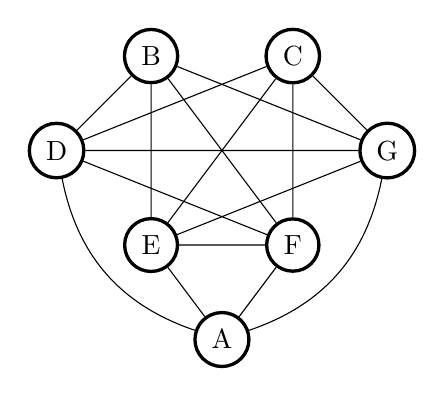
\begin{tikzpicture} 
         [scale=1.2,auto=left,every node/.style={circle,draw, very thick}]
         \node (b) at (1,3)  {B}; 
         \node (c) at (2.5,3)  {C}; 
         \node (d) at (0,2)  {D}; 
         \node (e) at (1,1)  {E}; 
         \node (f) at (2.5,1)  {F}; 
         \node (g) at (3.5,2)  {G}; 
         \node (a) at (1.75,0)  {A};
         \foreach \from/\to in {b/d, b/e, b/f, b/g, d/c, d/g, d/f, e/c,
         e/g, e/f, f/c, g/c, a/e, a/f} 
            \draw (\from) -- (\to);    
         \draw[bend left] (a) to (d);
         \draw[bend right] (a) to (g);
       \end{tikzpicture}     
  \end{center}

  Um emparelhamento $E$ de $G$ nos da uma opção de jogos que podemos
  fazer em um dia, uma vez que cada vértice tem no máximo uma aresta de
  $E$ incidindo sobre ele e as duas pontas dessa aresta devem jogar uma
  contra a outra. Um outro emparelamento $E'$, disjunto de $E$
  nos da outra opção de de jogos que poderiam ser feitos em outro dia, e
  assim por diante.
  Portanto, precisamos do menor número de emparelhamentos disjuntos não
  vazios de
  forma a cobrir todas as arestas de $A(G)$. Em outras paralvras,
  precisamos encontrar uma coloração das arestas de $G$ com o menor
  número de cores possível. Dessa forma, o índice cromático de $G$ deve
  nos dar a quatidade de dias necessários para realizar todos os jogos.\\
  O grafo $G$ possui $16$ arestas e podemos ver que $\Delta(G) = 5$.
  Assim, $$|A(G)| = 16 > \frac{1}{2}\Delta(G)(n-1) = \dfrac{1}{2}\cdot5\cdot6 =
  15$$
  Portanto, pelo resultado de \textbf{E27} e pelo \textbf{Teorema 6.3}
  temos que $\chi'(G) = \Delta(G)+1 = 6$. Portanto são necessários $6$
  dias para realizar os jogos nas condições dadas. Uma possível divisão
  desses jogos poderia ser realizada da seguinte forma:
\begin{center} 
     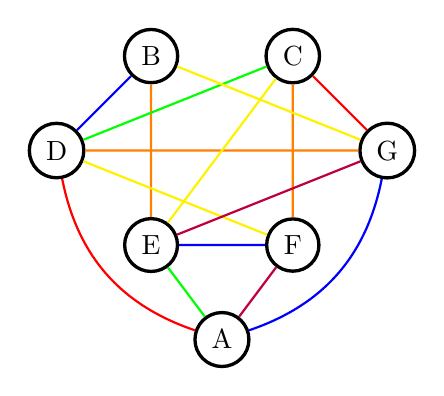
\begin{tikzpicture} 
         [scale=1.2,auto=left,every node/.style={circle,draw, very thick}]
         \node (b) at (1,3)  {B}; 
         \node (c) at (2.5,3)  {C}; 
         \node (d) at (0,2)  {D}; 
         \node (e) at (1,1)  {E}; 
         \node (f) at (2.5,1)  {F}; 
         \node (g) at (3.5,2)  {G}; 
         \node (a) at (1.75,0)  {A};
         \foreach \from/\to in {b/e, c/f, d/g}
            \draw[color=orange, thick] (\from) -- (\to);    
         \foreach \from/\to in {d/c, e/a}
            \draw[color=green, thick] (\from) -- (\to);
         \foreach \from/\to in {d/f, e/c, b/g}
            \draw[color=yellow, thick] (\from) -- (\to);
         \foreach \from/\to in {e/g, a/f}
            \draw[color=purple, thick] (\from) -- (\to);
         \foreach \from/\to in {e/f, b/d}
            \draw[color=blue, thick ] (\from) -- (\to);
         \draw[color=red, thick] (c) to (g);   
         \draw[bend left, color=red, thick] (a) to (d);
         \draw[bend right, color=blue, thick] (a) to (g);
       \end{tikzpicture}
       \hspace{50px}
\begin{tabular}{|c|c|}
\hline
\textbf{Dia} & \textbf{Cor} \\ \hline
1º           & Vermelho     \\ \hline
2º           & Amarelo      \\ \hline
3º           & Verde        \\ \hline
4º           & Roxo         \\ \hline
5º           & Azul         \\ \hline
6º           & Laranja      \\ \hline
\end{tabular}
  \end{center}
  Na figura, cada cor representa quais jogos serão realizados num
  determinado dia. A correpondência entre cores e
  dias é mostrada na tabela.

\paragraph{E29.} Cinco pessoas devem participar de um campeonato
de \textit{bridge}:\medskip\\
Abel (A), Beto (B), Carlos (C), Duda (D) e Enzo (E).\medskip\\
Um jogo de \textit{bridge} é jogado entre times formados por 2 pessoas.
Todo time VW deve jogar contra todos os demais oturos times XY
distintos (ou seja, U, V, X e Y devem ser 2 a 2 distintos). Note que
os times não são fixos: podemos ter times AB, AC, AD, AE, ..., e cada
um desses times deve jogar contra todos os demais (claramente não ao
mesmo momento). Expressar cada time pelas iniciais dos nomes em ordem
alfabética.\medskip\\
\textcolor{red}{Se o mesmo time não pode jogar 2 vezes num memso
dia}, qual é o menor número de dias para a realização do
campeonato? Descreva como o problema pode ser formulado como um problema
sobre grafos, diga como é o grafo, qual é o menor número de dias
(justificando como concluiu isso), e apresente uma solução (uma tabela
dos jogos em cada um dos dias).
\paragraph{Soluçao:} Podemos traduzir essa questão para um problema
sobre grafos. O campeonato pode ser representado por um grafo $G$ onde
cada vértice de $V(G)$ é um time diferente e uma aresta $uv$ pertence
a $A(G)$ se e somente se os times $u$ e $v$ não tem membros em comum, ou
seja $u\cap v = \emptyset$.
Uma forma de desenha esse grafo é a seguinte:
\begin{center} 
     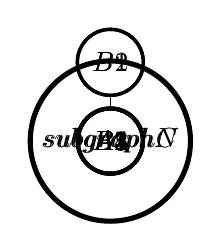
\begin{tikzpicture}[every node/.style={draw,circle,very thick}]
  \graph [clockwise,math nodes] {     
    subgraph C [V={ {AC}, {BD}, {CE}, {AB}, {DE} }, name=A, radius=3cm]; 
    subgraph N [V={ {BE}, {AE}, {AD}, {CD}, {BC} }, name=B, radius=1.5cm];
    \foreach \i [evaluate={\j=int(mod(\i+1,5)+1);}] in {1,...,5}{
      A \i -- B \i;  
      B \i -- B \j;
    }
  }; 
\end{tikzpicture} 
\end{center}\\
 Essa lei de formação do grafo resulta no \textbf{grafo de
 Petersen}. Assim como na questão anterior, emparelhamentos nos dão
 as opções de jogos que podemos fazer em um dia. Portanto,
 analogamente à questão anterior, o índice cromático desse grafo nos da
 o menor número de dias necessários para se realizar todos os jogos. O
 índice cromático do grafo de Petersen é bem conhecido e é 4. Portanto,
 com 4 dias é possível realizar todos os jogos. A tabela abaixo mostra
 como poderiam ser organizados esses jogos:
\begin{table}[h]
\centering
\begin{tabular}{|c|c|}
\hline
\textbf{Dia}              & \textbf{Jogos}                                             \\ \hline
{\color[HTML]{FE0000} 1º} & (AC vs BD); (BE vs CD); (BC vs AE); (DE vs AB); (AD vs CE) \\ \hline
{\color[HTML]{3166FF} 2º} & (AC vs DE); (BE vs AD); (AB vs CD); (BD vs CE)             \\ \hline
{\color[HTML]{F56B00} 3º} & (DE vs BC); (AC vs BE); (BD vs AE); (AB vs CE)             \\ \hline
{\color[HTML]{32CB00} 4º} & (BC vs AD); (CD vs AE)                                     \\ \hline
\end{tabular}
\end{table}
\end{document}

